\documentclass[10pt, a4paper]{report}
\usepackage[utf8]{inputenc}
\usepackage[T1]{fontenc}
%\usepackage[top=3cm,bottom=2cm,left=2cm,right=2cm]{geometry}
\usepackage[framed, numbered]{matlab-prettifier}
\usepackage{graphicx,epstopdf}
\usepackage{amsmath}
\usepackage{amsfonts}
\usepackage{amssymb}
\usepackage{graphics}
\usepackage{tikz}
\usepackage{amsbsy} % librerias ams
\usepackage[americanvoltages]{circuitikz}
\usepackage{verbatim} 
\usepackage{mathtools}
\usepackage{steinmetz}%polares
\usepackage{pdfpages}%pdf
\usepackage{float}% recuadro de figurafigure
\floatstyle{boxed} 

\title{Lab Experience V}
\author{Darwin R.  \thanks{funded by the Overleaf team}}
\date{\today}

\begin{document}


    \begin{titlepage}
    \maketitle
    \end{titlepage}
\section{Laboratorio IV.}
\begin{flushleft}
 
  Usando el Lugar Geométrico de las Raíces diseñar controladores en PD y PID, de tal forma que cumplan lo siguiente

Caso Subamortiguado según los polos asignados en la experiencia dos. Diseñar un
compensador PD y PID, de tal modo que se reduzca el sobrepico a la mitad.

\end{flushleft}
 
\begin{figure}[h]
  \centering
  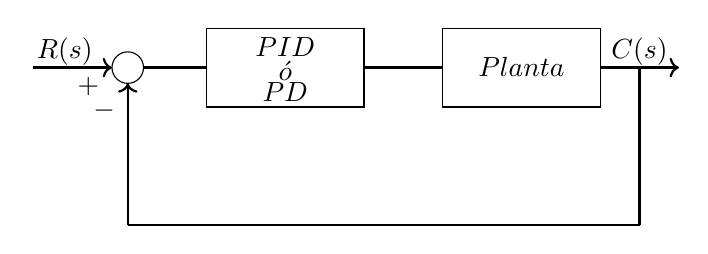
\begin{tikzpicture}
      %eje xn  n
      \draw[thick, ->](-0.2,1)--(0.8,1);
      \draw[thick, -](1.2,1)--(2,1);
      \draw[thick, -](4,1)--(5,1);
      \draw[thick, ->](7,1)--(8,1);
      \draw[thick, -] (7.5,1) -- (7.5,-1);
      \draw[thick, -] (7.5,-1) -- (1,-1);
      \draw[thick, ->] (1,-1) -- (1,0.8);
      \draw (2,0.5) rectangle (4,1.5);
      \draw (5,0.5) rectangle (7,1.5);
      \draw (1,1) circle (0.2);
      \node[below] at (3,1.51){$PID$};
      \node[below] at (3,1.21){$\acute{o} $};
      \node[below] at (3,0.93){$PD$};
      %planta
      \node[below] at (6,1.25){$Planta$};
      %signos
      \node[below] at (0.5,1){$+$};
      \node[below] at (0.7,0.7){$-$};
      \node[below] at (0.2,1.5){$R(s)$};
      \node[below] at (7.5,1.5){$C(s)$};
      
  \end{tikzpicture}
  \caption[]{Diagrama de bloques.}
\end{figure}

Diseño de un controlador de PD. Circuito propuesto en la guía de experiencia.
\begin{figure}[htp]
  \centering
  \ctikzset{bipoles/resistor/height/.initial=.2}
  \ctikzset{bipoles/resistor/width/.initial=.5}
  \begin {circuitikz} [thick]
  \draw
    % Amplificador Operacional
  (5,2.5) node[op amp] (opamp) {\texttt{U1}}
    % Entrada E(s)
    (-2,3) node[above]{$E(s)$} to[short, o-] ++(1,0)
    (-1,1.495) node[]{}  ++(0,1.495)
    to[short] ++(0.5,0) to[R=$R_1$] ++(3.5,0) 
    (-1,1.495) node[]{}  ++(0,1.495)
    to[short] ++(0,1.459) to[C=$C_1$] ++(4,0)-| ++(0,-1.46) node[circ]{}
    to[short] ++(0.8,0)  ++(1,-0.46) %-| ++(0,-1.46) node[circ]{}
    (7,2.5) node[above]{$G(s)$} to[short, o-] ++(-0.8,0) -| ++(0,2) -| ++(-0.2,0) to[R=$R_2$] ++(-2.4,0) -| ++(0,-1.495) node[circ]{}
    (opamp.+) -| ++(0,-1) node[ground]{}
    ;
  \end{circuitikz}
  \caption[]{Circuito del compensador.}
\end{figure}
  

    \begin{equation}
      \frac{E(s)-0}{Z_{in}}=\frac{0-G(s)}{R_2}
    \end{equation}

    \begin{equation}
      Z_{in}=\frac{R_1}{1+R_1 C_1 s}
    \end{equation}

    \begin{equation*}
      \begin{split}
      \frac{G(s)}{E(s)}=\frac{-R_2(1+R_1 C_1 s)}{R_1} \\
      \frac{G(s)}{E(s)}=-\frac{R_2 R_1 C_1(s+ \frac{1}{R_1 C_1})}{R_1}
      \end{split}
    \end{equation*}
       \begin{equation}
        \frac{G(s)}{E(s)}=-R_2 C_1 (S +\frac{1}{R_1 C_1})
       \end{equation}
    \begin{equation}
      \frac{G(s)}{E(s)}= K_{p} T_{d}(S+\frac{1}{T_{d}})
    \end{equation}

    Una vez determinada la función de transferencia del compensador, se aprecia que aporta un cero a la función de transferencia y un valor proporcional. El aporte del cero hace que las raíces se dirigen más al eje imaginario por lo que hace que el sistema sea más estable, puede apreciarse mejor en la figura 3.
Desarrollando el circuito proporcional integrativo, de la figura 2.


\begin{figure}[h]
  \centering
  \begin{tikzpicture}[scale=0.5]
      %eje x
      \draw[densely dotted, ->](-4.3,0)--(0.5,0) node[right]{$\sigma  $};
      \draw[thick,-](-8,0)--(-4.3,0) node[right]{};   
      %eje y
      
      \draw[thick, ->](-0.1,-4)--(-0.1,4) node[left]{$j\omega $};
      % etiquetas eje x 
      \foreach \x in {}
     \draw (\x, 0.1)--(\x, -0.1)node[below]{$\x$};
       % etiquetas eje y
       \foreach \y in {}
     \draw (0.1, \y)--(-0.1, \y)node[right]{$\y$};

       % componente en x
     \draw (-4.3,0) circle (0.1);
      \draw (-2.1,2) arc (40:316:3);
      \draw[densely dotted] (-2.2,-2) arc (-43:40:3);
      \node[left, blue] at (-1.6,2){$\times $};
      \node[left, blue] at (-1.7,-2){$\times $};
      
  \end{tikzpicture}
  \caption{Lugar de las raices de dos polos y un cero.}
\end{figure}



Con respecto a los polos asignados, se tiene los siguientes datos.\\
Polos:
\begin{equation*}
  \rho_{1,2}=-1\pm 2i
\end{equation*}
Función de transferencia:
\begin{equation*}
  G(s)=\frac{C(s)}{R(s)}=\frac{5}{S^2 +2S +5}
\end{equation*}
Constante de amortiguamiento:
\begin{equation*}
  \xi=0.4472135
\end{equation*}
Frecuancia natural no amortiguada:
\begin{equation*}
  \begin{split}
    \omega_{n}&=\sqrt{5}\hspace{0.1cm} rad/s\\
    \omega_{n}&=2.236067977 \hspace{0.1cm} rad/s  
  \end{split}
\end{equation*}
Frecuancia natural amortiguada:
\begin{equation*}
  \begin{split}
    \omega_{d}&= \omega_{n} \sqrt{1-\xi ^2}\\
    \omega_{d}&= 2 \hspace{0.1cm} rad/s
  \end{split}
\end{equation*}
Máximo sobre impulso:
\begin{equation*}
  \begin{split}
    MP &= e^{-(\frac{\xi}{\sqrt{1-\xi^2}})\pi }\\
    MP &= 0.20787 \hspace{0.1cm} 
  \end{split}
\end{equation*}
Para sistemas realimentados.
Para sistemas realimentados se aprecia que existe un error de estado estable, este
error se reduce si se coloca un valor proporcional, pero esto a su vez reduce el
valor de la constante de amortiguamiento, por lo que el sobrepico se incrementa y
esto no es favorable.
\begin{equation*}
  G(s)=\frac{C(s)}{R(s)}=\frac{5k}{S^2 +2S +5k}
\end{equation*}
\begin{figure}[htp]
  \centering
  \includegraphics[width=0.7\linewidth]{epsfile1.eps}
  \caption{Respuesta de sistemas.}
  \label{fig:espfig}
\end{figure}
\lstinputlisting[style=Matlab-editor,basicstyle=\mlttfamily\scriptsize, caption={Código en Matlab.}]{respuestasincomoensador.m}
%
De la figura 4 para la respuesta el lazo cerrado aparte del error de establecimiento, la
respuesta se hace más rápida , por ejemplo el tiempo pico de la respuesta en lazo cerrado
es de 1s frente a 1.5s de la respuesta en lazo abierto.
Determinado el nuevo valor de la constante de amortiguamiento, partiendo de las
condiciones de lazo abierto.
Reduciendo a un 50$\%$ el sobrepico máximo.
\begin{equation*}
  \begin{split}
    MP &= e^{-(\dfrac{\xi}{\sqrt{1-\xi^2}})\pi }\\
    MP &= 0.1 \hspace{0.1cm} \\
    \xi &=\sqrt{\frac{(ln(MP))^2}{\pi^2 + (ln(MP))^2}}\\
    \xi &=0.5
  \end{split}
\end{equation*}

como se explico antes , el lazo cerrado la respuesta es más rápida por lo que reducimos el tiempo pico , y de esa forma tener una forma de condicionar el valor de la frecuencia no amortiguada.

\begin{equation*}
  \begin{split}
  t_{s} & = 0.5 \\
  t_{s} & = \frac{3.7}{ \xi  \omega_{n}} \\
  t_{s} & = 0.5 = \frac{3.7}{0.59  \omega_{n}}\\
  \omega_{n} & =12.5423 \hspace{0.1cm} rad/s
  \end{split}
\end{equation*}
Con el valor de la frecuencia no amortiguada determinamos la frecuencia amortiguada.
\begin{equation*}
  \begin{split}
    \omega_{d} &= \omega_{n} \sqrt{1-\xi^2}\\
    \omega_{d} &= 10.1267 \hspace{0.1cm} rad/s
  \end{split}
\end{equation*}
con estos datos se puede obtener los puntos del nuevo polo. que satisface los
anteriores requerimientos.
\begin{equation}
\rho_{1,2}=- \xi \omega_{n} \pm \omega_{d} i 
%\rho_{1,2}=- \xi \omega_{n} \pm \omega_{d} i
\end{equation}%

\begin{equation*}
\rho_{1,2}=- 7.4 \pm 10.1267 i
\end{equation*}
Con este punto determinamos el compensador PD , utilizando las condicones
que ofrecen el lugar de las raices.

\begin{figure}[htp]
  \centering
  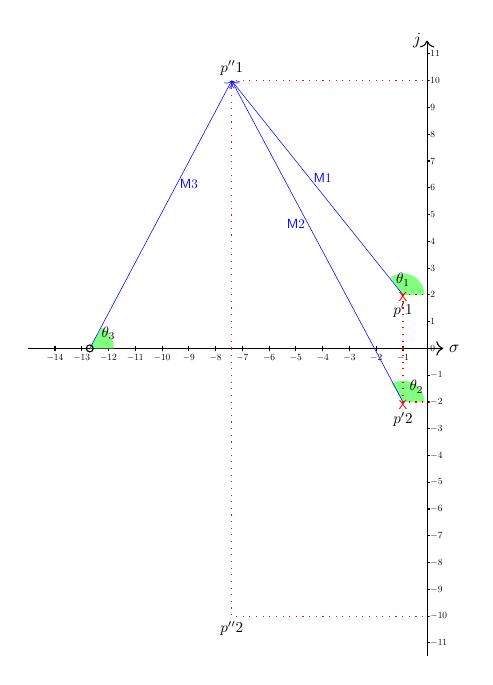
\begin{tikzpicture}[scale=0.34,transform shape]
      %eje x
      \draw[thin, ->](-15,0)--(0.5,0) node[right,scale=1.8]{$\sigma  $};
      %eje y
      
      \draw[thin, ->](-0.1,-11.5)--(-0.1,11.5) node[left,scale=1.8]{$j$};
      % etiquetas eje x
     \foreach \x in {-14,...,-1}
     \draw (\x, 0.1)--(\x, -0.1)node[below]{$\x$};
       % etiquetas eje y
     \foreach \y in {11,...,-11}
     \draw (0, \y)--(-0.1, \y)node[right]{$\y$};
       % componente en x
       \fill[green!50!white] (-1,2) -- (-0.2,2) arc (0:126:0.8) -- (-1,2);
       \fill[green!50!white] (-1,-2) -- (-0.2,-2) arc (0:121:0.8) -- (-1,-2);
       \fill[green!50!white] (-12.7,0) -- (-11.8,0) arc (0:60:0.9) -- (-12.3,0.7);
       %\draw (-13,0) -- (-7.4,10) arc (40:319:15.3) -- (-13,0);
        \draw[thin,dotted, red](-1,0)--(-1,2);
        \node[below,scale=1.6] at (-1,1.9){$p'1$};
        \draw[thin,dotted, red](-1,0)--(-1,-2);
        %\node[above] at (-1,-2){$Vx$};
       % componente en y
      \draw[thin,dotted, red](0,2)--(-1,2);
      \node[below,scale=1.6] at (-1,-2.2){$p'2$};
      \draw[thin,dotted, red](0,-2)--(-1,-2);
      
      %-------------------------------------------
       % componente en x
       \draw[thin,dotted, red](-7.4,0)--(-7.4,10);
       \node[above,scale=1.6] at (-7.4,10){$p''1$};
       \draw[thin,dotted, red](-7.4,0)--(-7.4,-10);
       
      % componente en y
     \draw[thin,dotted, red](0,10)--(-7.4,10);
     \node[below,scale=1.6] at (-7.4,-10){$p''2$};
     \draw[thin,dotted, red](0,-10)--(-7.4,-10);
    
      %Vector
      \draw[very thin, blue, ->](-1,2)--(-7.4,10);
      \draw[ very thin, blue, ->](-1,-2)--(-7.4,10);
      \draw[ very thin, blue, ->](-12.7,0)--(-7.4,10);
      \node[below, blue,scale=1.4] at (-4,6.7){$\mathsf{M} 1$};
      \node[below, blue,scale=1.4] at (-5,5){$\mathsf{M} 2$};
      \node[below, blue,scale=1.4] at (-9,6.5){$\mathsf{M} 3$};
      \node[below,scale=1.6] at (-1,3){$\theta_{1}$};
      \node[below,scale=1.6] at (-0.5,-1){$\theta_{2}$};
      \node[below,scale=1.6] at (-12,1){$\theta_{3}$};
      \node[below,red,scale=1.4] at (-1,2.26){$\mathsf{X}  $};
      \node[below,red,scale=1.4] at (-1,-1.75){$\mathsf{X}  $};
      \draw (-12.7,0) circle (0.13cm);
  \end{tikzpicture}
  \caption{Lugar de las raices de polos y el cero en el punto de prueba.}
\end{figure}

Los ángulos de los polos en lazo abierto con respecto al polo de prueba.
\begin{equation*}
  \begin{split}
    \theta_1 &= 180^{\circ} - \arctan \frac{8.12}{6.4}\\
    \theta_1 &= 128.24^{\circ}\\
    \theta_2 &= 180^{\circ} - \arctan \frac{12.12}{6.4}\\
    \theta_2 &= 117.83^{\circ}
  \end{split}
\end{equation*}

\begin{equation*}
 % \begin{split}
   % 
   \textup{Deficiencia del ángulo}= 128.24^{\circ} + 117.83^{\circ} - 180^{\circ} = 66.07^{\circ}
   % \ph\min ase{\frac{5}{S^2 +2S +5}}= \pm  180^{\circ} \scriptstyle (2k+1)(k=0,1,2,...)
  %\end{split}
\end{equation*}
\begin{equation*}
    \theta_3 = 66.07^{\circ}
 \end{equation*}
 Con ese ángulo determinamos la ubicación del cero, de tal forma que solucione el desfase.
 \begin{equation*}
  \begin{split}
  \tan (66.07)&= \frac{12.12}{x -7.4}\\
  x &= 12.77
  \end{split}
 \end{equation*}
 donde X es la ubicación de cero, entonces el nuevo valor de cero es:
 \begin{equation*}
   (S+12.77)
 \end{equation*}
%z = 1.19 \phase{-78.2039}
  Determinando las magnitudes.
  \begin{equation*}
    \begin{split}
    M_1 = 10.3389\\
    M_2 = 13.7059\\
    M_3 = 11.447\\
      %
    \left\lvert \frac{K M_3 5 }{M_2 M_1}\right\rvert_{\rho_{1,2}=-7.4\pm 10.1267i} = 1 \\
    K=2.4758
    \end{split}
  \end{equation*}
   con los datos obtenidos se forma el siguiente compensador.
   \begin{equation*}
     \frac{G(s)}{E(s)} = - R_2 C_1 (S+\frac{1}{R_1 C_1}) =- 2.4758(S+ 12.777)
   \end{equation*}
   Determinando los valores de los componentes.
   \begin{equation*}
     \begin{split}
       C_1&=680 \mu F\\
       R_1&=115.096 \Omega\\
       R_2&= 3.640 K \Omega 
     \end{split}
   \end{equation*}
  \floatstyle{boxed} 
   \restylefloat{figure}
    \begin{figure}[htp]
      \centering
      \includegraphics[trim={0 2cm 5cm 2cm},scale=0.4]{circuito1.pdf}
      \caption{Implementación del circuito.}
     
    \end{figure}

  
    \begin{figure}[htp]
      \centering
      \includegraphics[scale=0.4]{circuito2.pdf}
      \caption{Respuesta del sistema compensado.}
    
    \end{figure}
    Observación:
    Los polos asignados el base a los valores de lazo abierto, con los cuales se
    esperaba reducir el sobrepico a la mitad, no se pudo realizar, esto era de esperar
    por que existe un error de estado estacionario,el valor de la constante de
    amortiguamiento se ve afectada por el valor proporcional e indirectamente por la

    ubicación del cero. como se aprecia en la ecuación siguiente que representa la
función de transferencia en lazo cerrado.
\begin{equation*}
  G(s)= \frac{C(s)}{R(s)} = \frac{(x+S)5K}{S^2 + S(2+5K) + 5 +aK5}
\end{equation*}
Para asegurar la reducción del sobrepico colocaremos un valor de constante de
amortiguamiento alto , también consideramos un tiempo pico mucho menor , esto
reduce el tiempo de respuesta producido por el incremento de K, generando
también un incremento en el valor de la ubicación del cero.\\

Recalculando de la misma forma, en anterior procedimiento.
\begin{equation*}
  \begin{split}
    \xi = 0.85\\
    t_s = 0.25 = \frac{3.7}{0.85 \omega_n}\\
    \omega_n = 17.411\\
    \omega_d = 9.1722
  \end{split}
\end{equation*}
El nuevo punto objetivo es:
\begin{equation*}
  \rho_{1,2}= -14.499 \pm 9.1722i
\end{equation*}
Determinado ángulo de desfase.
\begin{equation*}
  \begin{split}
    \theta_1 &= 180^{\circ} - \arctan \frac{7.1722}{13.794}\\
    \theta_1 &= 152.52^{\circ}\\
    \theta_2 &= 180^{\circ} - \arctan \frac{11.1722}{12.794}\\
    \theta_2 &= 140.994^{\circ}
  \end{split}
\end{equation*}
\begin{equation*}
  % \begin{split}
    % 
    \textup{Deficiencia del ángulo}= 152.52^{\circ} + 140.994^{\circ} - 180^{\circ} = 113.5225^{\circ}
    % \ph\min ase{\frac{5}{S^2 +2S +5}}= \pm  180^{\circ} \scriptstyle (2k+1)(k=0,1,2,...)
   %\end{split}
 \end{equation*}
 \begin{equation*}
     \theta_3 = 113.5225^{\circ}
  \end{equation*}
  Con ese ángulo determinamos la ubicación del cero, de tal forma que solucione el desfase.
  \begin{equation*}
   \begin{split}
   \tan (113.5225)&= \frac{9.1722}{x -14.799}\\
   x &= 10.8068
   \end{split}
  \end{equation*}
  donde X es la ubicación de cero, entonces el nuevo valor de cero es:
  \begin{equation*}
    (S+10.8068)
  \end{equation*}
  Determinando las magnitudes.
  \begin{equation*}
    \begin{split}
    M_1 = 15.551\\
    M_2 = 17.7547\\
    M_3 = 10.0033\\
      %
    \left\lvert \frac{K M_3 5 }{M_2 M_1}\right\rvert_{\rho_{1,2}=-14.799\pm 9.1722i} = 1 \\
    K=5.5202
    \end{split}
  \end{equation*}
   con los datos obtenidos se forma el siguiente compensador.
   \begin{equation*}
     \frac{G(s)}{E(s)} = - R_2 C_1 (S+\frac{1}{R_1 C_1}) =- 5.5202(S+ 10.8068)
   \end{equation*}
   Determinando los valores de los componentes.
   \begin{equation*}
     \begin{split}
       C_1&=680 \mu F\\
       R_1&=136.079 \Omega\\
       R_2&= 8.1179 K \Omega 
     \end{split}
   \end{equation*}
   \begin{figure}[htp]
    \centering
    \includegraphics[trim={0 3cm 5cm 2cm},scale=0.4]{circuito3.pdf}
    \caption{Implementación del circuito.}
   
  \end{figure}


  \begin{figure}[htp]
    \centering
    \includegraphics[scale=0.4]{circuito4.pdf}
    \caption{Respuesta del sistema compensado.}
  
  \end{figure}

  En base a incrementar el valor de la constante amortiguamiento y reducir el tiempo pico de acuerdo al comportamiento del sistema realimentado se logró reducir el sobrepico a la mitad y reducir considerablemente el error de estado estacionario.
  
  \begin{figure}[htp]
    \centering
    \includegraphics[width=0.7\linewidth]{untitled.eps}
    \caption{Respuesta de sistemas compensado.}
    \label{fig:espfig2}
  \end{figure}
  \lstinputlisting[style=Matlab-editor,basicstyle=\mlttfamily\scriptsize, caption={Código en Matlab.}]{respuestacc.m}
  %





\end{document}
